\chapter{New Coordination Geometries for \texorpdfstring{\ce{Re^I}}{Rhenium (I)}} \label{chap.newchem}
\markright{New Coordination Geometries for \texorpdfstring{\ce{Re^I}}{Rhenium (I)}} % new right header
%======================================================================
\section{Introduction}
%======================================================================

As mentioned previously in the thesis introduction, \ce{Re^I} compounds have been typically bidentate (\ce{$\kappa$^2}) compounds, even when using a potentially terdentate (\ce{$\kappa$^3}) ligand such as bis(imino)pyridine or terpyridine (refer to \autoref{fig.terdentateligands}). The chemistry of this rhenium $\alpha$-imino complex has been extensively invesigated, with over 1700 references appearing in a structure search for that metal-ligand motif. The extraction of an additional carbonyl and the chelation of the pendant arm of the ligand was attempted to extend the pi system of the ligand and its interaction with the metal centre. This was first demonstrated by prior work in our group for the bis(imino)pyridine ligand\autocite{jurca2013}. 

%======================================================================
\section{Synthesis of Bidentate and Terdentate \texorpdfstring{\ce{Re^I}}{Rhenium (I)} Complexes}
%======================================================================

Similar to the prior work, synthesis began with the production of the bidentate complex \ce{$\kappa$^2(terpy)Re(CO)3X} (X = Cl, Br) by coordination of 2,2':6',2''-terpyridine (Sigma) with a \ce{Re(CO)5X} (Strem) starting material in dry toluene at reflux for 4 hours, as shown in \autoref{scheme.bidentate}. A bright yellow powder precipitated from solution and was collected by filtration, washed with cold hexanes, and dried \textit{in vacuo} to a good yield of \textbf{1} and \textbf{3} respectively.\footnote{Experimental details for all compounds can be seen in \autoref{chap.exp} \nameref{chap.exp}} These bidentate compounds were characterized fully and used without further purification to produce \ce{$\kappa$^3(terpy)Re(CO)2X} (X = Cl, Br) via thermolysis, as well as for anion exchange reactions. 

\missingfigure{bidentate scheme}
\begin{scheme}[!htbp]
 \begin{center}
  
\includegraphics[clip=true]{images/insertgraphic.eps}
 \end{center}
\caption[Synthesis of \textbf{1} and \textbf{2}]{Synthesis of \textbf{1} and \textbf{2}}
\label{scheme.bidentate}
\end{scheme} 

Conversion of compounds \textbf{1} and \textbf{3} to the $\kappa ^3$ moiety required the release of \ce{CO} and the subsequent coordination of the free pendant arm. Prior work had identified the thermal lability of the carbonyl, based on a method first described by Buckingham with a osmium complexes\autocite{buckingham1964}. In this method, a ceramic sample boat was placed in a tube furnace at elevated temperature, under a flowing atmosphere of \ce{N2}. After some time, the sample is removed and collected at nearly quantitative yield. Determination of the appropriate thermolysis temperature was performed by \gls{ac.tga} of the sample. A 6-8 \% mass loss (dependant on sample) indicated the departure of one carbonyl group from the complex. Results of \gls{ac.tga} on \textbf{1} and \textbf{3} is shown in \autoref{fig.tga}. For \textbf{1}, thermolysis was performed at 240$^\circ$C, and for \textbf{3} thermolysis was performed at 260$^\circ$C\todo{check that value}, yielding \textbf{2} and \textbf{4} respectively, at quantitative yields.

\begin{figure}[!htbp]
 \begin{center}
  \includegraphics[clip=true, width=140mm]{images/tga.eps}
 \end{center}
\caption[Results of \glsentrytext{ac.tga} analysis on \textbf{1} and \textbf{3}]{Results of \glsentrytext{ac.tga} analysis on \textbf{1} and \textbf{3}}
\label{fig.tga}
\end{figure} 
\todo{Further discuss TGA \& terdentate rxn to build a space to put in scheme2}
\missingfigure{terdentate scheme2}

Further reactions were carried out on the above products to yield triflate and cyano complexes of bidentate and terdentate geometries. These anion exchange reactions were performed by the addition of the silver salt to \textbf{1} or \textbf{2}, to precipitate \ce{AgCl}, leaving \ce{$\kappa$^2(terpy)Re(CO)3CN} (\textbf{5}), \ce{$\kappa$^3(terpy)Re(CO)2CN} (\textbf{6}), \ce{$\kappa$^2(terpy)Re(CO)3OTf} (\textbf{7a}) and \ce{$\kappa$^3(terpy)Re(CO)2OTf} (\textbf{8a}), as shown in \autoref{scheme.anion}. Resulting in only moderate yields, \textbf{7b} and \textbf{8b} were synthesized by the direct addition of neat triflic acid (\ce{CF3SO3H}) to \textbf{1} and \textbf{2} respectively. \ce{HCl} was released, the solutions were quenched by addition of aqueous \ce{NaCO3}, and product was collected, again at moderate yield. 

\missingfigure{anion exchange reaction schemes}

\begin{scheme}[!htbp]
 \begin{center}
  
\includegraphics[clip=true]{images/insertgraphic.eps}
 \end{center}
\caption[Anion exchange pathways]{Anion exchange pathways to synthesize \textbf{3} - \textbf{8}8}
\label{scheme.anion}
\end{scheme} 

A pseudo-tridentate complex was targeted to compare \ce{CO2} photoreduction performace with the previously prepared catalysts. Typical \ce{[L2L$'$Re(CO)_n]+} (n = 2, 3) targets exchange the halide for a neutral phosphine or imine type ligand, resulting in a cationic species with weakly coordinated anion (typically \ce{BF4-}, \ce{OTf-}, \ce{BArF-} or other anion)\todo{ref}. Instead, we targeted the \ce{L2L$'$Re(CO)2Cl} (L = bipy, L$'$ = 4-\textit{t}-butylpyridine) compound (\textbf{9}) via two similar methods (\autoref{scheme.pseudo}).

\missingfigure{anion exchange reaction schemes}
\begin{scheme}[!htbp]
 \begin{center}
  
\includegraphics[clip=true]{images/insertgraphic.eps}
 \end{center}
\caption[Synthesis of pseudo-tridentate]{Synthesis of \ce{L2L$'$Re(CO)2Cl} (L = bipy, L$'$ = 4-\textit{t}-butylpyridine) (\textbf{9})}
\label{scheme.pseudo}
\end{scheme} 

%======================================================================
\section{Characterization}
%======================================================================

Characterization was performed on each of the products synthesized as discussed above. \Gls{ac.nmr} analysis, x-ray crystallography, as well as UV-Vis and IR spectroscopy was performed. Computational \gls{ac.dft} methods were used to solve the geometries, and \gls{ac.tddft} was performed to predict UV-Vis spectra and identify electronic transitions. 

%----------------------------------------------------------------------
\subsection{NMR Analysis}
%----------------------------------------------------------------------

Proton \gls{ac.nmr} was performed on each of the samples. Each sample was dissolved completely in deuteroacetonitrile (\ce{CD3CN}) and analysis was performed on a Bruker AVANCE 400 MHz spectrometer. Data was processed from the FID signal via the TopSpin program, and spectra were analyzed using ACD NMR Processor v12.0. 

Detailed peak analysis comparing bidentate samples \textbf{1}, \textbf{3}, \textbf{5}, and \textbf{7} or terdentate \textbf{2}, \textbf{4}, \textbf{6}, and \textbf{8} show little difference between samples. This is due to the distance between the anion and any protons on the ligand. While anions with different $\sigma$ donor strength marginally impact the metal-ligand interactions, these have only small effect on the location of peaks, shifting between samples by typically less than 0.1 ppm. As is shown in \autoref{fig.bid3nmr}, the characteristic shape of each spectra remains constant, only exact peak locations and some peak order varies with anion choice. 

\missingfigure{S6 from paper, nmr of 2,3,4}
\begin{figure}[!htbp]
 \begin{center}
  
\includegraphics[clip=true]{images/insertgraphic.eps}
 \end{center}
\caption[The aromatic region of the \texorpdfstring{\ce{^1H}}{1H} \glsentrytext{ac.nmr} spectra of 3 bidentate compounds]{The aromatic region of the \texorpdfstring{\ce{^1H}}{1H} \glsentrytext{ac.nmr} spectra for compounds \textbf{•} (red), \textbf{•} (green), and \textbf{•}(blue)}
\label{fig.bid3nmr}
\end{figure} 
\todo{check compounds \& spectra}

The characteristic feature in the \gls{ac.nmr} spectra after the transformation from bidentate to terdentate (e.g. sample \textbf{1} to \textbf{2}) is the simplification of the signals in the aromatic region (between 7 and 9 ppm). This simplification is due to the increased symmetrization of the ligand, while the \ce{$\kappa$^2} bidentate ligand has a freely rotating pendant group, the \ce{$\kappa$^3} terdentate ligand is in a more rigidly fixed geometry. Prior work in literature\todo[color=red]{Get paper citation} and in our group\todo[color=red]{Titel's Thesis citation} shows the temperature dependence of the rate of rotation of this pendant arm for various ligand species. 

\missingfigure{S5 from paper, showing bi-terdentate}
\begin{figure}[!htbp]
 \begin{center}
  
\includegraphics[clip=true]{images/insertgraphic.eps}
 \end{center}
\caption[The aromatic region of the \texorpdfstring{\ce{^1H}}{1H} \glsentrytext{ac.nmr} spectra showing bidentate - terdentate conversion]{The aromatic region of the \texorpdfstring{\ce{^1H}}{1H} \glsentrytext{ac.nmr} spectra for compounds \textbf{•} (red) and \textbf{•}(blue), showing the simplification of the spectra upon the conversion from bidentate to terdentate}
\label{fig.bidtoter}
\end{figure} 
\todo{check compounds \& spectra}

The simplification of peaks due to the symmetrization of the ligand results in the peaks from () and ()\todo{Put in nmr peak values} aligning with their mirror peaks at () and (). \autoref{fig.terpynmr} shows the proton expanded ligand, the peaks at () and () correspond with the protons () and (). 

\missingfigure{expanded terpy}
\begin{figure}[!htbp]
 \begin{center}
  
\includegraphics[clip=true]{images/insertgraphic.eps}
 \end{center}
\caption[Proton-explicit skeletal drawing of 2,2':6',2''-terpyridine]{Proton-explicit skeletal drawing of 2,2':6',2''-terpyridine}
\label{fig.terpynmr}
\end{figure} 

Carbon \gls{ac.nmr} (\ce{^{13}C}) was attempted on the complexes as well. Unfortunately, \ce{Re^I} complexes perform poorly in \ce{^{13}C} \gls{ac.nmr} experiments, the signal to noise ratio is incredibly poor (if a signal is even visible). The effect of this is a lack of \ce{^{13}C} \gls{ac.nmr} analysis of these compounds in literature, with a very few exceptions. \todo{why poor, show an ok result \& discuss}

%----------------------------------------------------------------------
\subsection{Structure Analysis with X-Ray Crystallography and DFT}
%----------------------------------------------------------------------

Single crystal analysis by x-ray crystallography yielded good structures of compounds \textbf{1}, \textbf{2}, \textbf{3}, \textbf{4}, \todo{the rest of structures}. These are the first reported crystal structures of the $\kappa ^3$ terdentate \ce{Re^I} compounds. A number of structural characteristics are common between the various bidentate or terdentate complexes. Much analysis has been done on the structures of bidentate complexes in literature\todo{ref}, the notable characteristic within terpyridine compounds is the rotation of the pendant arm pushing the nitrogen atom away from the plane of the metal-ligand bonds by approximately 100$^\circ$. Cell parameters and other collection data for compounds \textbf{1}, \textbf{3}, \textbf{5}, and \textbf{7} are located in \autoref{tab.bidxraycp}.

In addition, the structures of all species were optimized using Gaussian 09\autocite{gaussian} employing the B3LYP\autocite{becke1993, lee1988}  exchange-correlation (XC) functional. The LanL2DZ basis set/effective core potential\autocite{hay1985} was used on Re and, the all-electron TZVP basis set\autocite{schafer1994} for the remaining lighter atoms. Frequency analysis of all structures was used to confirm the nature of the stationary points. Solvent effects were computed when necessary using the integral equation formalism variant of the \gls{ac.pcm} for solvation within Gaussian 09\autocite{tomasi2005, scalmani2006}.The results of these calculations are compared to the x-ray crystallography data in the tables below.

\todo[inline]{Compare xray to computational structures in tables and discussions}

Sample \textbf{3}'s crystal structure had a higher symmetry than the other samples. Details on the exact methods used for structure elucidation are available in \autoref{sec.xray}, but all of the structures found are of high quality. The structures of \textbf{1}, \textbf{3}, and \textbf{5} can be seen in \autoref{fig.da1}, \autoref{fig.da3} and \autoref{fig.da5}, respectively, and more views of these structures can be seen in \autoref{sec.xray}. Crystals suitable for x-ray analysis were unable to be collected from compound \textbf{7}. 

\begin{figure}[!htbp]
 \begin{center}
  \includegraphics[clip=true, width=60mm, height=60mm, keepaspectratio]{images/xray1a.eps}
 \end{center}
\caption[X-ray crystal structure representation for \textbf{1}.]{X-ray crystal structure representation for \textbf{1}. Only one of the two of the molecules in the unit cell are shown. Co-crystallized chloroform, hydrogen atoms, and thermal ellipsoids of ligand carbon atoms are omitted for clarity.}
\label{fig.da1}
\end{figure}

\begin{figure}[!htbp]
 \begin{center}
  \includegraphics[clip=true, width=60mm, height=60mm, keepaspectratio]{images/xray3a.eps}
 \end{center}
\caption[X-ray crystal structure representation for \textbf{3}.]{X-ray crystal structure representation for \textbf{3}. Co-crystallized chloroform, hydrogen atoms, and thermal ellipsoids of ligand carbon atoms are omitted for clarity.}
\label{fig.da3}
\end{figure}

\begin{figure}[!htbp]
 \begin{center}
  \includegraphics[clip=true, width=60mm, height=60mm, keepaspectratio]{images/xray5a.eps}
 \end{center}
\caption[X-ray crystal structure representation for \textbf{5}.]{X-ray crystal structure representation for \textbf{5}. Only one of the two of the molecules in the unit cell are shown. Co-crystallized chloroform, hydrogen atoms, and thermal ellipsoids of ligand carbon atoms are omitted for clarity.}
\label{fig.da5}
\end{figure}

Selected bond lengths, bond angles, and torsions are listed in \autoref{tab.da1}, \autoref{tab.da3} and \autoref{tab.da5} for products \textbf{1}, \textbf{3}, and \textbf{5} respectively. The structures can be seen in \autoref{fig.da1}, \autoref{fig.da3} and \autoref{fig.da5}, and more views of these structures can be seen in \autoref{chap.exp}, \autoref{ssec.views}, \nameref{ssec.views}. 

The \ce{Re^I} centre in the pseudooctahedral complex is supported by a planar, pincer coordinated ligand defined by the terminal and central pyridyl group of the terpyridine. One of the carbonyl groups lies in this plane trans to the central pyridyl group, while the remaining carbonyl groups and the anionic group or other complexed species lie on an approximately perpindicular plane to the ligand. Bond angles around the Re centre show a significant deviation of up to 15$^\circ$ from the ideal octahedral geometry for all samples analyzed. The typical N-Re-N bond angle of 75$^\circ$ is due to the atomic size of rhenium, comparison to the crystal structure of an analogous compound with a manganese atom\autocite{compain2014} shows an increase in the bonding angle by approximately 4$^\circ$ due to a decrease of bond length from metal to nitrogen of about 0.12 \r{A} for both the central and terminal pyridines. 

The deviation from octahedral is further visible in the rotation of the X-Re-CO plane (X=halide, anion, complexed group) by approximately 10 degrees from the right angle relative to the plane of the ligand. The axial halide, anion, or chelated group typically occupies a position such that it is slightly eclipsing the ligand, when viewed from the axial position. This eclipsing is due to some unknown process, no steric interference exists upon that site, analysis of electostatic or other short-range electronic effects computationally show any interaction between this site and the aromatic rings. In \ce{Re^I} complexes, the halide or anion is located axial relative to the plane of the ligand. For the acetonitrile complex with triflate counterion, the acetonitrile occupies the axial position. This site occupation holds through the complete set of x-ray crystal structures with a \ce{$\kappa$^2-(bipy)Re(CO)3X} core structure motif deposited in the \gls{ac.ccdc} database\autocite{allen2002}, and extends through other $\alpha$-diimine complexes seen in our lab and in literature\autocite{jurca2013}. 

The crystal structure for compound \textbf{5} contains two molecules per unit cell, one of which is solved to have the cyano group in the position trans to the ligand. However, careful analysis of the bond lengths, angles, and torsion data in \autoref{tab.da5} shows a remarked similarity between all -CO and -CN groups. Additionally, in an x-ray diffraction pattern, -CN and -CO look quite similar. Thus, while the structure solved to the two isomers, critical analysis would suggest that this molecule does not violate the axial position pattern laid out above. The computed structures energies in \autoref{tab.cneng} show a favouring of the axial position by 12-16 kJ/mol in the gas phase and by \gls{ac.pcm} in a simulated acetonitrile solvent. 

% Table generated by Excel2LaTeX
\begin{table}[!h]
\centering
 \begin{threeparttable}
  \caption{Solvated and gas phase energy differences between Axial \& Trans geometries of \ce{$\kappa$^x-(terpy)-Re(CO)_{5-x}CN} (x=2,3)}
    \begin{tabular}{cccc}
    \toprule
    \multicolumn{2}{c}{Bidentate} & \multicolumn{2}{c}{Terdentate} \\ \midrule
    E(gas)\tnote{a} & E(solution)\tnote{b} & E(gas)\tnote{a} & E(solution)\tnote{b} \\ \midrule
    14.70 & 11.87 & 16.28 & 16.43 \\
    \bottomrule
    \end{tabular}%
    \begin{tablenotes}
    \item [a] B3LYP SCF energy in kcal/mol.
    \item [b] B3LYP SCF energy in kcal/mol, with PCM solvation in acetonitrile.
    \end{tablenotes}
  \label{tab.cneng}%
 \end{threeparttable}
\end{table}%




Selected bond lengths, bond angles, and torsions are listed in \autoref{tab.da1}, \autoref{tab.da3} and \autoref{tab.da5} for products \textbf{1}, \textbf{3}, and \textbf{5} respectively.

% Table generated by Excel2LaTeX
\begin{table}[htbp]
  \caption{Selected Distances, Angles, and Torsions for \textbf{1}}
  \centering
    \begin{tabular}{ccc}
    \toprule
    \multirow{2}{*}{Bond} & \multicolumn{2}{c}{Distance (\r{A})} \\ \cline{2-3}
     & Experimental & Calculated \\ \midrule
    Re(1)-C(16) & 1.89(1) & 1.916 \\
    Re(1)-C(17) & 1.934(8) & 1.936 \\
    Re(1)-C(18) & 1.90(1) & 1.918 \\
    Re(1)-N(1) & 2.162(6) & 2.197 \\
    Re(1)-N(2) & 2.236(9) & 2.293 \\
    Re(1)-Cl(1) & 2.496(2) & 2.525 \\ \midrule
    \multirow{2}{*}{Angle} & \multicolumn{2}{c}{Degrees ($^\circ$)} \\ \cline{2-3}
     & Experimental & Calculated \\ \midrule
    C(16)-Re(1)-C(17) & 87.6(4) & 86.877 \\
    C(16)-Re(1)-C(18) & 88.3(4) & 90.613 \\
    C(17)-Re(1)-C(18) & 87.3(4) & 89.557 \\
    C(16)-Re(1)-N(1) & 96.4(3) & 96.240 \\
    C(17)-Re(1)-N(1) & 174.9(3) & 175.600 \\
    C(18)-Re(1)-N(1) & 95.9(3) & 93.506 \\
    C(16)-Re(1)-N(2) & 169.3(3) & 170.368 \\
    C(17)-Re(1)-N(2) & 101.1(3) & 102.755 \\
    C(18)-Re(1)-N(2) & 98.3(3) & 89.415 \\
    N(2)-Re(1)-N(1) & 74.5(3) & 74.146 \\
    C(16)-Re(1)-Cl(1) & 91.7(3) & 91.453 \\
    C(17)-Re(1)-Cl(1) & 91.7(3) & 94.786 \\
    C(18)-Re(1)-Cl(1) & 179.9(3) & 175.286 \\
    N(1)-Re(1)-Cl(1) & 84.0(2) & 82.058 \\
    N(2)-Re(1)-Cl(1) & 81.6(2) & 87.840 \\
    O(1)-C(16)-Re(1) & 179.6(9) & 178.224 \\
    O(2)-C(17)-Re(1) & 176.0(8) & 176.907 \\ 
    O(3)-C(18)-Re(1) & 177.3(9) & 179.317 \\ \midrule
    \multirow{2}{*}{Torsion} & \multicolumn{2}{c}{Degrees ($^\circ$)} \\ \cline{2-3}
     & Experimental & Calculated \\ \midrule
    N(1)-C(5)-C(6)-N(2) &  16(1) & 15\\
    N(2)-C(10)-C(11)-N(3) & 41(1) & 139\\
    \bottomrule
    \end{tabular}%
  \label{tab.da1}%
\end{table}%



% Table generated by Excel2LaTeX
\begin{table}[htbp]
  \caption{Selected Distances, Angles, and Torsions for \textbf{2.3}}
  \centering
    \begin{tabular}{ccc}
    \toprule
   \multirow{2}{*}{Bond} & \multicolumn{2}{c}{Distance (\r{A})} \\ \cline{2-3}
     & Experimental & Calculated \\ \midrule
    Re(1)-C(16) & 1.911(3) & 1.91740 \\
    Re(1)-C(17) & 1.890(3) & 1.91814 \\
    Re(1)-C(18) & 1.921(4) & 1.93897 \\
    Re(1)-N(1) & 2.173(3) & 2.19687 \\
    Re(1)-N(2) & 2.232(2) & 2.28998 \\
    Re(1)-Br(1) & 2.6410(4) & 2.67953 \\ 
    C(16)-O(1) & 1.150(4) & 1.15290 \\
    C(17)-O(2) & 1.157(4) & 1.15012 \\
    C(18)-O(3) & 1.155(5) & 1.15591 \\ \midrule
    \multirow{2}{*}{Angle} & \multicolumn{2}{c}{Degrees ($^\circ$)} \\ \cline{2-3}
     & Experimental & Calculated \\ \midrule
    C(16)-Re(1)-C(17) & 89.1(1) & 90.772 \\
    C(16)-Re(1)-C(18) & 85.9(1) & 86.823 \\
    C(16)-Re(1)-N(1) & 97.9(1) & 96.034 \\
    C(17)-Re(1)-N(1) & 92.5(1) & 93.597 \\
    C(18)-Re(1)-N(1) & 175.4(1) & 175.575 \\
    C(16)-Re(1)-N(2) & 171.2(1) & 170.290 \\
    C(17)-Re(1)-N(2) & 96.0(1) & 89.435 \\
    C(18)-Re(1)-N(2) & 101.3(1) & 102.886 \\
    N(1)-Re(1)-N(2) & 74.7(1) & 74.265 \\
    C(16)-Re(1)-Br(1) & 92.7(1) & 90.399 \\
    C(17)-Re(1)-Br(1) & 177.6(1) & 176.076 \\
    C(18)-Re(1)-Br(1) & 91.6(1) & 94.069 \\
    N(1)-Re(1)-Br(1) & 85.74(7) & 82.555 \\
    N(2)-Re(1)-Br(1) & 82.07(7) & 88.780 \\
    O(1)-C(16)-Re(1) & 178.6(3) & 178.270 \\
    O(2)-C(17)-Re(1) & 179.5(3) & 179.355 \\
    O(3)-C(18)-Re(1) & 179.9(3) & 176.781 \\\midrule
    \multirow{2}{*}{Torsion} & \multicolumn{2}{c}{Degrees ($^\circ$)} \\ \cline{2-3}
     & Experimental & Calculated \\ \midrule
    N(1)-C(6)-C(1)-N(2) & -15.4(4) & -14.749 \\
    N(2)-C(5)-C(11)-N(3) & 141.1(3) & 136.119 \\
    \bottomrule
    \end{tabular}%
  \label{tab.da3}%
\end{table}%



% Table generated by Excel2LaTeX
\begin{table}[htbp]
  \caption{Selected Distances, Angles, and Torsions for \textbf{5}}
  \centering
    \begin{tabular}{cccc}
    \toprule
    \multicolumn{4}{c}{Selected Distances (\r{A})} \\ \midrule
    \multicolumn{2}{c}{Cyanide Axial} & \multicolumn{2}{c}{Cyanide Trans} \\ \midrule
    Re(2)-C(35) & 2.148(7) & Re(1)-C(19) & 2.105(8) \\
    Re(2)-C(36) & 1.926(6) & Re(1)-C(16) & 1.928(5) \\
    Re(2)-C(37) & 1.954(7) & Re(1)-C(18) & 1.96(1) \\
    Re(2)-C(38) & 1.902(9) & Re(1)-C(17) & 1.918(7) \\
    Re(2)-N(5) & 2.242(7) & Re(1)-N(1) & 2.253(5) \\
    Re(2)-N(6) & 2.168(5) & Re(1)-N(2) & 2.176(4) \\
    C(35)-N(8) & 1.138(9) & C(19)-O(3) & 1.17(1) \\
    C(36)-O(4) & 1.145(8) & C(16)-N(4) & 1.149(7) \\
    C(37)-O(5) & 1.151(9) & C(18)-O(2) & 1.14(1) \\
    C(38)-O(6) & 1.17(1) & C(17)-O(1) & 1.130(8) \\ \midrule
    \multicolumn{4}{c}{Selected Angles (deg)} \\ \midrule
    \multicolumn{2}{c}{Cyanide Axial} & \multicolumn{2}{c}{Cyanide Trans} \\ \midrule
    C(16)-Re(1)-C(17) & 87.8(3) & C(36)-Re(2)-C(38) & 87.7(3) \\
    C(16)-Re(1)-C(18) & 87.0(3) & C(36)-Re(2)-C(37) & 88.0(3) \\
    C(16)-Re(1)-C(19) & 92.5(3) & C(36)-Re(2)-C(35) & 92.1(3) \\
    C(17)-Re(1)-C(18) & 88.7(3) & C(38)-Re(2)-C(37) & 88.5(3)\\
    C(17)-Re(1)-C(19) & 90.5(3) & C(38)-Re(2)-C(35) & 90.8(3)\\
    C(18)-Re(1)-C(19) & 179.1(3) & C(37)-Re(2)-C(35) & 179.2(3) \\
    C(16)-Re(1)-N(1) & 102.2(2) & C(36)-Re(2)-N(5) & 100.6(3) \\
    C(16)-Re(1)-N(2) & 175.9(2) & C(36)-Re(2)-N(6) & 174.2(3) \\
    C(17)-Re(1)-N(1) & 168.3(3) & C(38)-Re(2)-N(5) & 169.3(3) \\
    C(17)-Re(1)-N(2) & 95.9(3) & C(38)-Re(2)-N(6) & 96.6(3) \\
    C(18)-Re(1)-N(1) & 97.7(3) & C(37)-Re(2)-N(5) & 98.4(2) \\
    C(18)-Re(1)-N(2) & 94.8(3) & C(37)-Re(2)-N(6) & 96.0(2) \\
    C(19)-Re(1)-N(1) & 83.2(2) & C(35)-Re(2)-N(5) & 82.3(2) \\
    C(19)-Re(1)-N(2) & 85.7(2) & C(35)-Re(2)-N(6) & 83.9(2) \\
    N(1)-Re(1)-N(2) & 73.9(2) & N(5)-Re(2)-N(6) & 74.7(2) \\
    O(1)-C(17)-Re(1) & 178.2(7) & O(6)-C(38)-Re(2) & 179.4(7) \\
    O(2)-C(18)-Re(1) & 172.0(7)& O(5)-C(37)-Re(2) & 175.5(6) \\ 
    O(3)-C(19)-Re(1) & 178.0(6) & N(8)-C(35)-Re(2) & 178.0(6) \\
    N(4)-C(16)-Re(1) & 178.7(6) & O(4)-C(36)-Re(2) & 179.0(7) \\ \midrule
    \multicolumn{4}{c}{Selected Torsions (deg)} \\ \midrule
    \multicolumn{2}{c}{Cyanide Axial} & \multicolumn{2}{c}{Cyanide Trans} \\ \midrule
    N(1)-C(1)-C(6)-N(2) & 12.5(8) & N(5)-C(20)-C(25)-N(6) & 14.5(9) \\
    N(1)-C(5)-C(11)-N(3) & 43.7(9) & N(5)-C(24)-C(30)-N(7) & 41(1) \\
    \bottomrule
    \end{tabular}%
  \label{tab.da5}%
\end{table}%



% Table generated by Excel2LaTeX

\begin{table}[!htb]
  \caption{Crystal data and structure refinement for compounds \textbf{2.1}, \textbf{2.3}, and \textbf{2.5}}
  \resizebox{\textwidth}{!}{%
  \begin{tabular}{rp{3.2cm}p{3.2cm}p{3.2cm}}
    \toprule
    Compound & \textbf{2.1} & \textbf{2.3} & \textbf{2.5}  \\
    \cmidrule(l){2-4} 
    Empirical formula & \ce{C19H11N3O3ReCl} & \ce{C19H11N3O3ReBr} & \ce{C20H11N4O3Re} \\
    Formula weight (g/mol) & 538.96 & 583.41 & 530.04 \\
    Temperature (K) & 200 & 200 & 200 \\
    Wavelength (\r{A})  & 0.71073 & 0.71073 & 0.71073 \\
    Crystal System & Triclinic & Monoclinic & Triclinic \\
    Space Group & P-1 & C2/c & P-1  \\
    a (\r{A}) & 9.8736(4) & 31.1537(7) & 9.9196(9) \\
    b (\r{A}) & 14.8202(4) & 7.1176(2) & 14.9902(14) \\
    c (\r{A}) & 16.3472(4) & 16.8519(4) & 16.5187(15) \\
    $\alpha$ (deg) & 69.2890(10) & 90.000 & 68.363(2) \\
    $\beta$ (deg) & 80.801(2) & 111.0230(10) & 80.929(2) \\
    $\gamma$ (deg) & 79.836(2) & 90.000 & 79.975(2) \\
    Volume (\r{A}\textsuperscript{3}) & 2190.00(12) & 3488.00 & 2236.6(4) \\
    Z, r (calc) (Mg/m\textsuperscript{3}) & 2, 1.997 & 8, 2.222 & 2, 1.927 \\
    Absorption coefficient (mm\textsuperscript{-1}) & 6.063 & 9.282 & 5.821 \\
    Absorption correction  & \multicolumn{3}{c}{Semi-empirical from equivalents} \\
    Final R indices [I$\geq$2$\sigma$(I)] & R1 = 0.0397,\newline wR2 = 0.0839 & R1 = 0.0232,\newline wR2 = 0.0614 & R1 = 0.0390,\newline wR2 = 0.0921 \\
    R indices (all data) & R1 = 0.0604,\newline wR2 = 0.0951 & R1 = 0.0285,\newline wR2 = 0.0642 & R1 = 0.0500,\newline wR2 = 0.0961 \\
    \bottomrule
  \end{tabular}} 
  \label{tab.bidxraycp}%
\end{table}%



\FloatBarrier

Structural comparisons between the bidentate samples and the terdentate show many similarities. The loss of one carbonyl always accompanies the dentation of the pendant arm of the ligand. The increased coordination forces the ligand to adopt a more rigidly planar geometry, this is visible in the structure of \textbf{2} (\autoref{fig.da2}) and \textbf{8} (\autoref{fig.da8}). Structures for other discusses species were unable to be collected.

\begin{figure}[!ht]
 \begin{center}
  \includegraphics[clip=true, width=60mm, height=60mm, keepaspectratio]{images/xray2a.eps}
 \end{center}
\caption[X-ray crystal structure representation for \textbf{2}.]{X-ray crystal structure representation for \textbf{1}. Only one of the two of the molecules in the unit cell are shown. Co-crystallized chloroform, hydrogen atoms, and thermal ellipsoids of ligand carbon atoms are omitted for clarity.}
\label{fig.da2}
\end{figure}

\begin{figure}[!ht]
 \begin{center}
  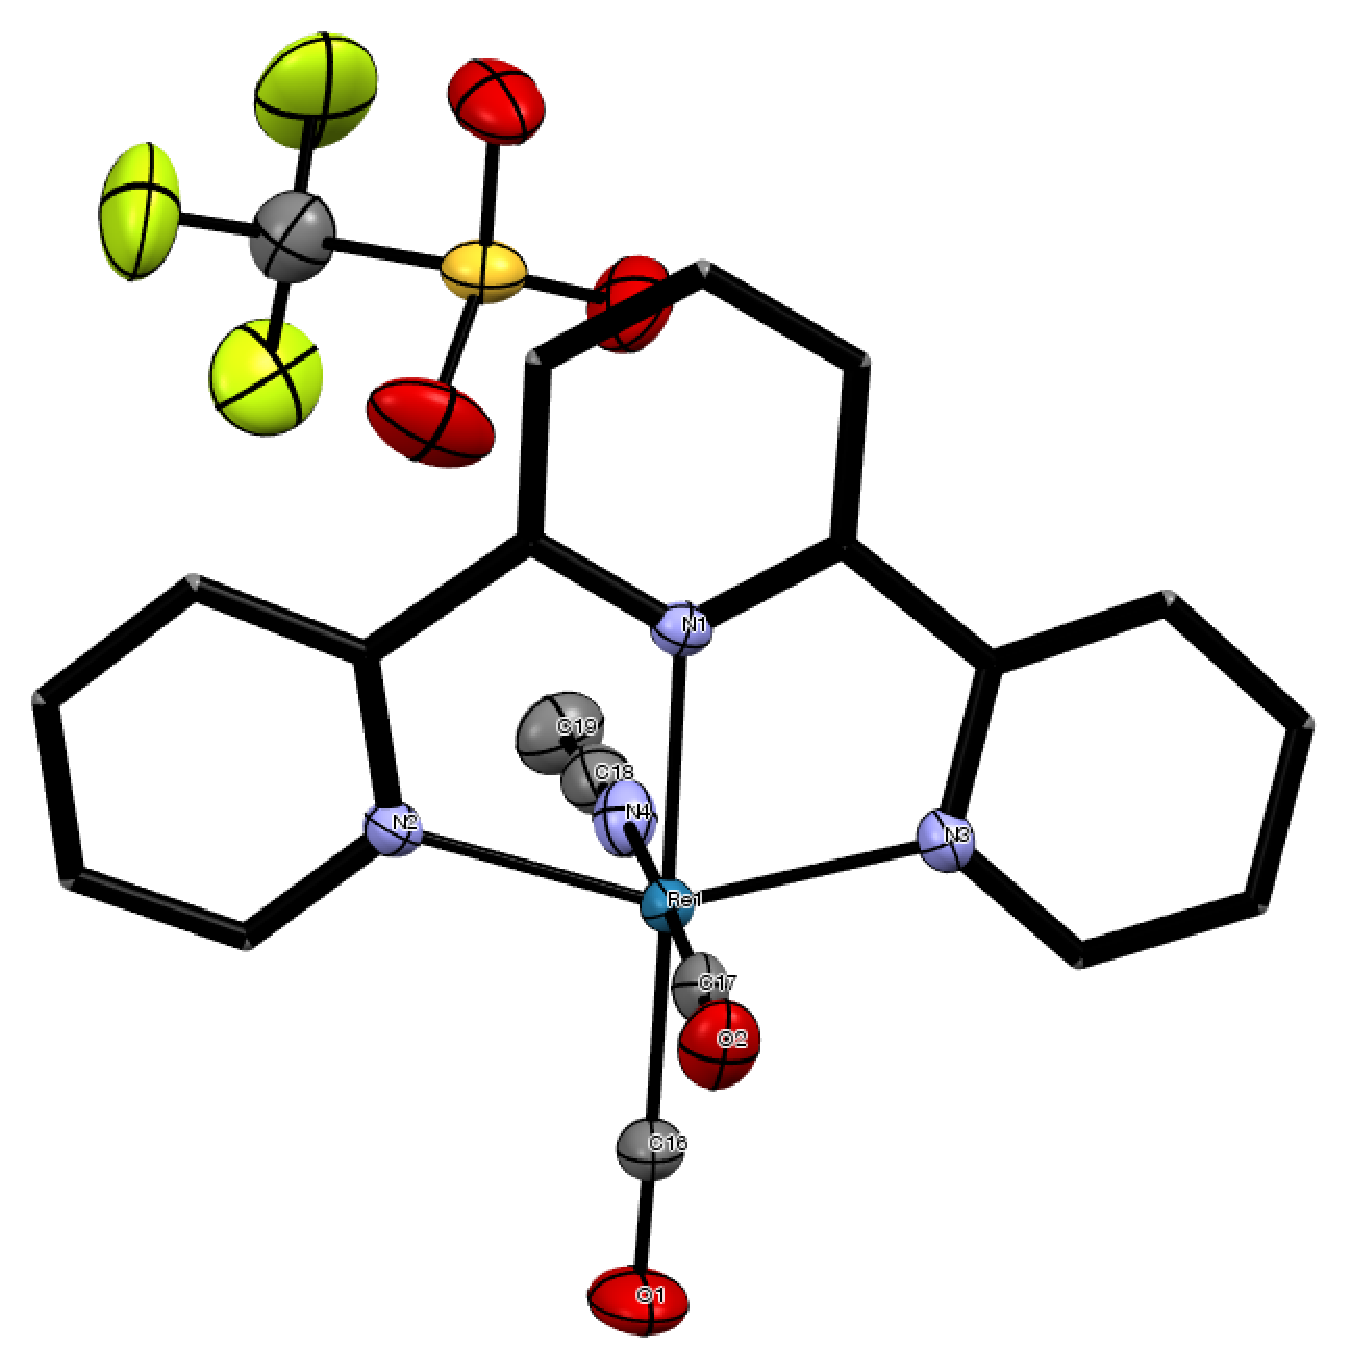
\includegraphics[clip=true, width=60mm, height=60mm, keepaspectratio]{images/xray8a.eps}
 \end{center}
\caption[X-ray crystal structure representation for \textbf{8}.]{X-ray crystal structure representation for \textbf{3}. Co-crystallized chloroform, hydrogen atoms, and thermal ellipsoids of ligand carbon atoms are omitted for clarity.}
\label{fig.da8}
\end{figure}

Selected bond lengths, bond angles, and torsions are listed in \autoref{tab.da2} and \autoref{tab.da8} for products \textbf{2} and \textbf{8}. Cell parameters and collection data can be found in \autoref{tab.terxraycp}. \todo{not done}

% Table generated by Excel2LaTeX
\begin{table}[htbp]
  \caption{Selected Distances, Angles, and Torsions for \textbf{2.2}}
  \centering
    \begin{tabular}{ccc}
    \toprule
    \multirow{2}{*}{Bond} & \multicolumn{2}{c}{Distance (\r{A})} \\ \cline{2-3}
     & Experimental & Calculated \\ \midrule
    Re(1)-C(16) & 1.926(9) & 1.92438\\
    Re(1)-C(17) & 1.975(10) & 1.90687\\
    Re(1)-N(1) & 2.119(7) & 2.13186\\
    Re(1)-N(2) & 2.080(7) & 2.08705\\
    Re(1)-N(3) & 2.126(7) & 2.13185\\
    Re(1)-Cl(1) & 2.489(3) & 2.53337 \\
    N(1)-N(3) & 4.14(1) & 4.14772 \\ 
    C(16)-O(1) & 1.14(1) & 1.16042 \\
    C(17)-O(2) & 1.05(1) & 1.16341 \\ \midrule
    \multirow{2}{*}{Angle} & \multicolumn{2}{c}{Degrees ($^\circ$)} \\ \cline{2-3}
     & Experimental & Calculated \\ \midrule
    C(16)-Re(1)-C(17) & 91.5(4) & 89.188 \\
    C(16)-Re(1)-N(2) & 173.7(4) & 172.050 \\
    C(17)-Re(1)-N(2) & 94.6(3) & 98.762 \\
    C(16)-Re(1)-N(1) & 103.9(3) & 102.980 \\
    C(17)-Re(1)-N(1) & 92.7(3) & 93.429 \\
    N(2)-Re(1)-N(1) & 77.3(3) & 76.684 \\
    C(16)-Re(1)-N(3) & 101.8(3) & 102.986 \\
    C(17)-Re(1)-N(3) & 91.7(3) & 93.419 \\
    N(2)-Re(1)-N(3) & 76.6(3) & 76.684 \\
    N(1)-Re(1)-N(3) & 153.7(3) & 153.210 \\
    C(16)-Re(1)-Cl(1) & 91.8(3) & 89.136 \\
    C(17)-Re(1)-Cl(1) & 176.5(2) & 178.324 \\
    N(2)-Re(1)-Cl(1) & 82.1(2) & 82.913 \\
    N(1)-Re(1)-Cl(1) & 85.4(2) & 86.953 \\
    N(3)-Re(1)-Cl(1) & 88.7(2) & 86.953 \\
    O(1)-C(16)-Re(1) & 177.9(9) & 179.079 \\
    O(2)-C(17)-Re(1) & 173.2(8) & 179.182 \\ \midrule
    \multicolumn{2}{c}{Selected Torsions (deg)} \\ \midrule
    N(1)-C(5)-C(6)-N(2) & 1(1) & 2 \\
    N(2)-C(10)-C(11)-N(3) & -4(1) & -2 \\
    \bottomrule
    \end{tabular}%
  \label{tab.da2}%
\end{table}%



% Table generated by Excel2LaTeX from sheet 'Sheet3'
\begin{table}[htbp]
  \centering
  \caption{Selected Distances, Angles and Torsions for Acetonitrile Adduct of \textbf{2.8}}
    \begin{tabular}{ccc}
    \toprule
	\multirow{2}{*}{Bond} & \multicolumn{2}{c}{Distance (\r{A})} \\ \cline{2-3}
     & Experimental & Calculated \\ \midrule
    Re(1)-C(16) & 1.889(4) & 1.93046 \\
    Re(1)-C(17) & 1.885(3) & 1.92844 \\
    Re(1)-N(1) & 2.091(3) & 2.10116 \\
    Re(1)-N(2) & 2.135(3) & 2.15397 \\
    Re(1)-N(3) & 2.131(3) & 2.15392 \\
    Re(1)-N(4) & 2.160(3) & 2.15202 \\ 
    N(2)-N(3) & 4.138(4) & 4.18483 \\ 
    C(16)-O(1) & 1.170(4) & 1.15749 \\
    C(17)-O(2) & 1.171(4) & 1.15244 \\ \midrule
	\multirow{2}{*}{Angle} & \multicolumn{2}{c}{Degrees ($^\circ$)} \\ \cline{2-3}
     & Experimental & Calculated \\ \midrule
    C(16)-Re(1)-C(17) & 87.69(16) & 88.104 \\
    C(16)-Re(1)-N(1) & 175.95(12) & 176.094 \\
    C(17)-Re(1)-N(1) & 96.35(12) & 95.802 \\
    C(16)-Re(1)-N(3) & 103.81(13) & 103.594 \\
    C(17)-Re(1)-N(3) & 94.03(12) & 92.309 \\
    N(1)-Re(1)-N(3) & 76.20(10) & 76.306 \\
    C(16)-Re(1)-N(2) & 103.58(13) & 103.598 \\
    C(17)-Re(1)-N(2) & 93.73(12) & 92.307 \\
    N(1)-Re(1)-N(2) & 75.99(10) & 76.305 \\
    N(3)-Re(1)-N(2) & 151.77(11) & 152.544 \\
    C(16)-Re(1)-N(4) & 90.50(14) & 88.484 \\
    C(17)-Re(1)-N(4) & 178.10(12) & 176.587 \\
    N(1)-Re(1)-N(4) & 85.46(10) & 87.611 \\
    N(3)-Re(1)-N(4) & 86.94(10) & 88.504 \\
    N(2)-Re(1)-N(4) & 86.15(10) & 88.485 \\
    O(1)-C(16)-Re(1) & 179.1(3) & 178.807 \\
    O(2)-C(17)-Re(1) & 178.0(3) & 178.860 \\\midrule
    \multirow{2}{*}{Torsion} & \multicolumn{2}{c}{Degrees ($^\circ$)} \\ \cline{2-3}
     & Experimental & Calculated \\ \midrule
    N(1)-C(1)-C(6)-N(2) & 1.7(4) & 1.105 \\
    N(1)-C(5)-C(11)-N(3) & -1.8(4) & -1.110 \\
    \bottomrule
    \end{tabular}%
  \label{tab.da8}%
\end{table}%

% Table generated by Excel2LaTeX
\begin{table}[!htb]
\centering
  \caption{Crystal data and structure refinement for compounds \textbf{2.2} and \textbf{2.8}}
    \begin{tabular}{rp{3.2cm}p{3.2cm}}
    \toprule
    Compound & \textbf{2.2} & \textbf{2.8} \\
    \cmidrule(l){2-3} 
    Empirical formula& \ce{C18H11N3O2ReCl} & \ce{C21H14N4O5F3SRe} \\
    Formula weight (g/mol) & 510.95 & 665.61 \\
    Temperature (K) & 200 & 200 \\
    Wavelength (\r{A}) & 0.71073 & 0.71073 \\
    Crystal System & Triclinic & Triclinic \\
    Space Group & P-1 & P-1 \\
    a (\r{A}) & 8.5275(3) & 8.5745(4) \\
    b (\r{A}) & 14.2421(5) & 11.9805(5) \\
    c (\r{A}) & 17.4637(6) & 13.0970(5) \\
    $\alpha$ (deg) & 77.948(2) & 79.748(2) \\
    $\beta$ (deg) & 85.684(2) & 81.106(2) \\
    $\gamma$ (deg) & 79.890 & 88.091(2) \\
    Volume (\r{A}\textsuperscript{3}) & 2041.79(12) & 1307.99(10) \\
    Z, r (calc) (Mg/m\textsuperscript{3}) & 4, 2.050 & 2, 1.993 \\
    Absorption coefficient (mm\textsuperscript{-1}) & 6.494 & 5.094 \\
    Absorption correction  & \multicolumn{2}{c}{Semi-empirical from equivalents} \\
    Final R indices [I$\geq$2$\sigma$(I)] & R1 = 0.0636,\newline wR2 = 0.1018 & R1 = 0.0294,\newline wR2 = 0.0673 \\
    R indices (all data) & R1 = 0.0985,\newline wR2 = 0.1110 & R1 = 0.0366,\newline wR2 = 0.0700 \\
    \bottomrule
    \end{tabular}%
  \label{tab.tercellparams}%
\end{table}%

\FloatBarrier

%----------------------------------------------------------------------
\subsection{Infrared Spectroscopy}
%----------------------------------------------------------------------

Conversion of bidenate to terdentate species was confirmed utilizing \gls{ac.ftir} spectroscopy. A small sample of powder product was placed on the Agilent Cary 630 \gls{ac.ftir} instrument, with \todo{get more info} and for a .

Analysis of the results shows the loss of one peak in the (ca.) 2000 \ce{cm^{-1}} region. This peak is in the CO stretching frequency, the frequency of the peak lost in thermolysis is indicative of a weakly coordinated carbonyl group. A shift occurs for one peak in the conversion from bidentat to terdentate, from 1890 to 1790 \ce{cm^{-1}}, indicating the further weakening of the metal carbonyl bonds remaining in the complex. This weakened bond is likely the carbonyl co-planar to the ligand, analysis of the x-ray crystal structure shows the CO bond to be 0.1 \r{A} longer than that of the axial carbonyl. Further analysis of the spectra were not successful in identification of any additional molecular properties, with the exception of a series of strong peaks appearing in the 1200-1300 \ce{cm^{-1}} range, confirming the presence of the triflate anion from the -\ce{SO3} group vibrations. 

\begin{figure}[!htbp]
 \begin{center}
  \includegraphics[clip=true, width=\textwidth]{images/ftir1and2.eps}
 \end{center}
\caption[FTIR Spectra for complexes \textbf{1} and \textbf{2}]{FTIR Spectra for complexes \textbf{1} (blue) and \textbf{2} (red).}
\label{fig.ir1}
\end{figure} 

%----------------------------------------------------------------------
\subsection{Photophysical Properties}
%----------------------------------------------------------------------

A striking observation upon the conversion of the bidentate species into the terdentate complexes is that these new compounds have a substantially darker colour that reflects a significant change in the photophysical properties. This effect was investigated using a combination of UV-visible spectroscopy and \gls{ac.dft} modelling. The stronger  absorbance of the terdentate complexes compared to the bidentate precoursors is evident in the UV-Vis spectra of these species, and is presented in \autoref{fig.uvvisexps}. These spectra were obtained in \gls{ac.dmso} with approximate concetrations of 0.01 mM for bidentate, and an order of magnitude lower (0.001 mM) for the terdentate analogues. The tridentate complexes have more intense absorbance for higher energy ligand UV-based $\pi$-$\pi^\ast$ transitions (\textless 400 nm) and certainly a richer visible absorption profile that involve the d-$\pi^\ast$ transitions. These features are responsible for the colour change observed.

\begin{figure}[!htbp]
 \centering
 \begin{subfigure}[b]{0.49\textwidth}
  \includegraphics[clip=true, width=\textwidth]{images/bidentateuvvis.eps}
  \caption{Spectra for compounds \textbf{1}, \textbf{3}, \textbf{5}, and \textbf{7}}
  \label{fig.uvvisbids}
 \end{subfigure}
 \begin{subfigure}[b]{0.49\textwidth}
  \includegraphics[clip=true, width=\textwidth]{images/terdentateuvvis.eps}
  \caption{Spectra for compounds \textbf{2}, \textbf{4}, \textbf{6}, and \textbf{8}}
  \label{fig.uvvisters}
 \end{subfigure}
\caption[UV-Vis spectra for all compounds]{UV-Vis spectra for all compounds. Concentrations of bidentate complexes are 0.01 mM and terdentate complexes are 0.001 mM.}
\label{fig.uvvisexps}
\end{figure} 

More UVVIS discussion.

\todo[inline]{This will be longer. Should be lots of discussion about results differences. I need to a)highlight the importance of anion exchange, and then b) highlight the importance of bidentate vs. terdentate}


% - - - - - - - - - - - - - - - - - - - - - - - - - - - - - - - - - - -
\subsubsection{UV-Vis Spectroscopy}
% - - - - - - - - - - - - - - - - - - - - - - - - - - - - - - - - - - -

\todo[inline]{This will be longer. Should be lots of discussion about results differences. I need to a)highlight the importance of anion exchange, and then b) highlight the importance of bidentate vs. terdentate}

%----------------------------------------------------------------------
\section{Conclusions}
%----------------------------------------------------------------------

\todo[inline]{Conclusion shows that manipulations can be done, this affects the photophysical properties of the compounds and may affect the photochemical}

